\documentclass[11pt]{article}
\usepackage[a4paper,margin=2.3cm]{geometry}
\usepackage{amsmath,amssymb}
\usepackage{booktabs}
\usepackage{graphicx}
\usepackage{siunitx}
\usepackage[hidelinks]{hyperref}
\usepackage{xcolor}
\usepackage{enumitem}
\setlist{itemsep=2pt,topsep=4pt}
\sisetup{range-phrase=--}
\newcommand{\Msun}{M_\odot}
\newcommand{\Mdot}{\dot M}
\newcommand{\kes}{\kappa_{\rm es}}
\newcommand{\status}[1]{\textsf{\small\textcolor{black!60}{[#1]}}}

\title{Do quasi-star photospheres survive infall?\\[2pt]
\large A steady-state test of the MESA-QUEST ``Little Red Dot'' models}
\author{Working notes --- T.~Abel (KIPAC), computed with Claude}
\date{15 October 2026 \quad (draft for discussion)}

\begin{document}
\maketitle

\begin{abstract}
\noindent
Santarelli, Bellinger et al.\ (2026, ApJL 998, L4) model Little Red Dots (LRDs) as late-stage
quasi-stars: $\sim\!10^6\,\Msun$, fully convective envelopes around accreting black holes, with
$L=L_{\rm Edd}(\kes)$, $T_{\rm eff}\approx6000$\,K, $\log g\approx0$. Their spectra come from LTE ATLAS9 atmospheres.
We ask two questions. (i) Given their stated surface properties, is the photosphere plausibly in LTE?
(ii) Does the $\sim6000$\,K hydrostatic photosphere survive the external infall that the direct-collapse
scenario requires? We build a quasi-static Z\,=\,0 envelope model in Julia (Saha EOS, Rosseland
continuum opacity, MLT, point-mass black hole) and replace the grey photosphere by a free-fall accretion
shock. Without infall, the model reproduces their surface parameters to $\sim$15\% in $T_{\rm eff}$.
With infall we find two steady branches at every $\Mdot>0$ tested. One is an essentially unchanged
``extended'' star. The other is a ``compact'' star 2.5--55$\times$ smaller with a 16--60\,kK boundary, buried in an
infall that is optically thick even in LTE. The two branches approach each other and disappear (a fold) at
$\Mdot\approx9$--$10\,\Msun\,{\rm yr^{-1}}$ for $M_{\rm BH}/M=0.1$ and 20--25 for $0.01$ (for $\Mdot/f$ if the infall
arrives in streams covering a fraction $f$); above that no steady hydrostatic solution exists. The \emph{observed} photosphere is at 5700--7600\,K on both branches for $\Mdot\ge1\,\Msun\,{\rm yr^{-1}}$
($\approx12$\,kK at $\Mdot=0.3$ on the compact branch). On the compact branch, however, it lies in infalling gas,
and the LTE assumption is weakest exactly there. Simple rate estimates indicate that
hydrogen at the paper's photosphere is strongly radiatively controlled, i.e.\ non-LTE.
\end{abstract}

\paragraph{Status labels.} Throughout, \status{computed} means a result of the code described here;
\status{estimate} means an order-of-magnitude rate or budget estimate with textbook approximations;
\status{interpretation} means our reading of the results, not separately derived.

\section{Context: the MESA-QUEST LRD models}
The fiducial model of Santarelli et al.\ has $M=10^6\,\Msun$, $Z=0$, $L\simeq3.72\times10^{10}\,L_\odot
=L_{\rm Edd}(\kes)$, and at the onset of the late stage ($M_{\rm BH}/M\simeq0.1$) $T_{\rm eff}=6241$\,K and
$\log g=-0.003$. These values imply $R=(L/4\pi\sigma T_{\rm eff}^4)^{1/2}=1.15\times10^{16}$\,cm
($1.65\times10^5\,R_\odot$, 770\,AU) and $M=gR^2/G=0.99\times10^6\,\Msun$, which is self-consistent. Their
eq.~(5) normalises $t_{\rm KH}$ to $R=2\times10^4\,R_\odot$, a factor $\approx8$ smaller than the radius implied by their own
$L$ and $T_{\rm eff}$.

From the public repository (\texttt{andysantarelli/MESA-QUEST}, directory \texttt{qs\_LRD\_ApJL2026}) we
read the following \status{verified by reading inlists/source}:
\begin{itemize}
\item \texttt{MLT\_option='TDC'}, $\alpha_{\rm MLT}=0.8$, \texttt{use\_superad\_reduction=.false.} (no MLT++).
\item Default MESA grey $T$--$\tau$ outer boundary; no outer-boundary accretion.
\item $L_{\rm BH}=\alpha\,4\pi cGM_\star/\kappa$ with $\kappa$ taken in the innermost cell; $\alpha=1$, $\epsilon=0.1$.
\item Inner boundary at the saturated-convection radius (tabulated, \texttt{Ki\_tab.dat}) with a cavity mass added to the core.
\item \texttt{convergence\_ignore\_equL\_residuals=.true.} and an energy-conservation tolerance of $10^{99}$.
\item Synthetic spectra from the MESA \texttt{colors} module, nearest ATLAS9 grid point (LTE, metal-bearing; the
paper notes $\log g$ lies outside the grid for most models).
\end{itemize}

\section{Is the photosphere in LTE?}\label{sec:nlte}
We estimate conditions at $\tau=2/3$ for a pure H/He gas with $P=(2/3)g/\kappa$ and H$^-$, H bound-free
and electron-scattering opacity, and compare collisional with radiative rates for hydrogen
\status{estimate}. Collisional ionization from $n=2$ uses a Seaton-type rate; photoionization from $n=2$ uses
$J_\nu=B_\nu(T_{\rm eff})$ and Kramers cross sections; collisional de-excitation of H$\alpha$ uses a van
Regemorter rate.
\begin{center}
\begin{tabular}{lccc}
\toprule
 & quasi-star & same $T_{\rm eff}$, $\log g=1$ & same $T_{\rm eff}$, $\log g=4.4$ \\
\midrule
$n_e$ at $\tau=2/3$ (cm$^{-3}$) & $5\times10^{11}$ & $1\times10^{12}$ & $1.6\times10^{13}$ \\
H ionized fraction & 0.025 & 0.011 & $8\times10^{-4}$\\
$n=2$: $C_{\rm ion}/R_{\rm ion}$ & $2\times10^{-3}$ & $4\times10^{-3}$ & $5\times10^{-2}$\\
H$\alpha$: $C_{32}/A_{32}$ & $2\times10^{-3}$ & $4\times10^{-3}$ & $5\times10^{-2}$\\
$P_{\rm rad}/P_{\rm gas}$ & 0.2 & 0.04 & $2\times10^{-4}$\\
\bottomrule
\end{tabular}
\end{center}
The $n=2$ population, which controls the Balmer-continuum opacity and hence the Balmer break, is set by
radiative rather than collisional processes by a factor $\sim500$. Above the thermalisation depth one
expects overionization of $n=2$ relative to LTE. This is the regime in which NLTE departures in hydrogen are
already documented for A--F supergiants at $\log g\approx1$--2, and the quasi-star sits below that. The
Balmer break, the feature the paper reproduces most closely (3.97 vs.\ $3.92\pm0.03$ for UNCOVER-45924), is
therefore the least LTE-safe observable. These estimates do not tell us the sign or size of the NLTE
change; that needs an NLTE calculation.

Related numbers \status{estimate}: escape speed $v_{\rm esc}=\sqrt{2gR}=\sqrt2(GMg)^{1/4}\approx1500$\,km\,s$^{-1}$.
The strong-shock temperature for free-fall infall is $T_{\rm sh}=\tfrac{3}{16}\mu m_Hv_{\rm ff}^2/k\approx3\times10^7$\,K.
In LTE, H$_2$ is negligible at the photosphere: $n_{\rm H_2}/n_{\rm H}\sim4\times10^{-8}$ at 6200\,K, rising only to
$\sim10^{-3}$ at 3000\,K and becoming significant below $\sim2500$\,K at these densities.

\section{Model}\label{sec:model}
The code (\texttt{QuasiStarInfall.jl}) is quasi-static and spherically symmetric. A steady state is
justified because $t_{\rm KH}=GM^2/(RL)\approx5\times10^3$\,yr $\ll M/\Mdot\sim10^6$\,yr at $1\,\Msun$\,yr$^{-1}$.

\subsection{Equation of state}
The composition is $X=0.76$, $Y=0.24$, $Z=0$ (as in the MESA-QUEST inlist). We use an ideal gas of
H, H$^+$, He, He$^+$, He$^{2+}$, e$^-$ in LTE plus blackbody radiation. The Saha equations, with
$\lambda_e^{-3}\equiv(2\pi m_ekT/h^2)^{3/2}$, are
\begin{equation}
\frac{n_{\rm H^+}n_e}{n_{\rm H^0}}=\lambda_e^{-3}e^{-\chi_{\rm H}/kT},\qquad
\frac{n_{\rm He^+}n_e}{n_{\rm He^0}}=4\lambda_e^{-3}e^{-\chi_{\rm He\,I}/kT},\qquad
\frac{n_{\rm He^{2+}}n_e}{n_{\rm He^+}}=\lambda_e^{-3}e^{-\chi_{\rm He\,II}/kT},
\end{equation}
closed by charge neutrality (solved by bisection in $\ln n_e$). The pressure is
$P=(n_{\rm H}+n_{\rm He}+n_e)kT+aT^4/3$. The specific entropy is the Sackur--Tetrode sum plus radiation,
\begin{equation}
s=\frac{k}{\rho}\sum_i n_i\left[\frac52+\ln\!\left(\frac{g_i}{n_i}\Big(\frac{2\pi m_ikT}{h^2}\Big)^{3/2}\right)\right]
+\frac{4aT^3}{3\rho}.
\end{equation}
All thermodynamic derivatives are taken numerically in $(\ln\rho,\ln T)$, which stays well conditioned for
$\beta\equiv P_{\rm gas}/P\ll1$. With $\chi_\rho=\partial\ln P/\partial\ln\rho|_T$, $\chi_T=\partial\ln P/\partial\ln T|_\rho$,
$s_\rho=\partial s/\partial\ln\rho|_T$ and $s_T=\partial s/\partial\ln T|_\rho$:
\begin{equation}
\nabla_{\rm ad}=\Big(\chi_T-\chi_\rho\frac{s_T}{s_\rho}\Big)^{-1},\quad
\Gamma_1=\chi_\rho-\chi_T\frac{s_\rho}{s_T},\quad
\delta=\frac{\chi_T}{\chi_\rho},\quad
c_P=s_T-s_\rho\,\delta .
\end{equation}
\status{computed} Checks: the fully ionized gas$+$radiation $\Gamma_1(\beta)=(32-24\beta-3\beta^2)/(24-21\beta)$ is
reproduced to $10^{-5}$ for $\beta=0.5,0.1,0.01$. The limits $\nabla_{\rm ad}\to0.4$ (ideal gas) and $0.25$ (radiation)
are recovered. In the H ionization zone at $P_{\rm gas}\approx30$\,dyn\,cm$^{-2}$, $\Gamma_1$ drops to $\approx0.97$ at 8000\,K.

\subsection{Opacity}
We use the Rosseland mean
$\kappa_R^{-1}=\int(\kappa_\nu^{\rm abs}+\kappa_\nu^{\rm sc})^{-1}\partial_TB_\nu\,d\nu\big/\int\partial_TB_\nu\,d\nu$
on 4000 frequencies, from these continuum sources: Thomson scattering; H Rayleigh scattering; hydrogenic
bound-free from H\,I ($n\le12$) and He\,II ($n\le8$) with LTE level populations and Kramers cross sections
$\sigma_n=2.815\times10^{29}Z^4/(n^5\nu^3)$; He\,I ground-state bound-free; free-free on H$^+$, He$^+$, He$^{2+}$
($\propto Z^2n_en_iT^{-1/2}\nu^{-3}$, Gaunt factor 1); and H$^-$ bound-free and free-free (John 1988).
Stimulated emission is included. \textbf{No bound--bound lines and no molecules} are included. $\kappa_R$ is
therefore a lower bound near $10^4$--$10^5$\,K, where line opacity in OPAL-type tables can raise it by a factor of a few.
The table spans $\log T=3.3$--8.0 and $\log R=-12$--1 ($R=\rho/T_6^3$). \status{computed} Checks: high-$T$ limit
$\kappa_R\to0.350$ (vs.\ $0.2(1+X)=0.352$ for $m_p$ vs.\ $m_H$); H$^-$ bound-free peak
$4.0\times10^{-17}$\,cm$^2$ at 0.85\,$\mu$m.

\subsection{Envelope}
The envelope is hydrostatic, with constant $L=L_{\rm Edd}(\kes,M)$ carried from the central source, and a
point mass $M_{\rm BH}$ at the centre. We integrate inward in $x=\ln P$:
\begin{equation}
\frac{dr}{dx}=-\frac{Pr^2}{Gm\rho},\qquad \frac{dm}{dx}=4\pi r^2\rho\frac{dr}{dx},\qquad \frac{d\ln T}{dx}=\nabla,
\end{equation}
with $\nabla_{\rm rad}=3\kappa LP/(16\pi acGmT^4)$. In convective regions $\nabla$ follows from local MLT
(Böhm-Vitense; Kippenhahn \& Weigert eq.~7.18) with $\alpha_{\rm MLT}=0.8$, $\ell=\alpha H_P$:
\begin{equation}
(\xi-U)^3+\tfrac{8U}{9}\left(\xi^2-U^2-W\right)=0,\quad
U=\frac{3acT^3}{c_P\rho^2\kappa\ell^2}\sqrt{\frac{8H_P}{g\delta}},\quad W=\nabla_{\rm rad}-\nabla_{\rm ad},
\end{equation}
\begin{equation}
\nabla=\xi^2-U^2+\nabla_{\rm ad},\qquad v_c^2=\frac{g\delta\,(\xi-U)^2\ell^2}{8H_P}.
\end{equation}
The shooting condition is $m(r_{\rm in})=M_{\rm BH}$ at $r_{\rm in}=\varepsilon_{\rm in}R$, with $R$ found by scanning
$\log R$ and bisecting every sign change. We use a Dormand--Prince 5(4) integrator with relative tolerance $10^{-7}$.
We report the local Eddington factor $\Gamma=\kappa L/(4\pi cGm)$ for radiation alone and the MLT Mach number $v_c/c_s$.

\subsection{Outer boundary}
\textbf{No infall} (equivalent to MESA's default): Eddington grey photosphere at $\tau=2/3$,
\begin{equation}
T_b=T_{\rm eff},\qquad P_b=\tfrac23\Big(\frac{g}{\kappa_b}+\frac{F}{c}\Big)\ \Longleftrightarrow\
P_{{\rm gas},b}=\tfrac23\frac{g}{\kappa_b}\,(1-\Gamma_\kappa),\qquad \Gamma_\kappa=\frac{\kappa_bF}{cg}.
\end{equation}
\textbf{Spherical free-fall infall} onto a radiative shock at $R$. Upstream,
$\rho_{\rm in}(r)=\Mdot/(4\pi r^2v_{\rm ff})\propto r^{-3/2}$ with $v_{\rm ff}=(2GM/r)^{1/2}$. Momentum balance across the
shock and settling layer gives
\begin{equation}
P_b=\rho_{\rm in}v_{\rm ff}^2+\tfrac23\frac{g}{\kappa_b}+\frac{F_{\rm tot}}{c}\Big(\tau_{\rm in}+\tfrac23\Big),\qquad
T_b^4=\tfrac34\,T_L^4\Big(\tau_{\rm in}+\tfrac43\Big),
\end{equation}
with $T_L^4=L_{\rm tot}/(4\pi\sigma R^2)$ and $L_{\rm tot}=L+GM\Mdot/R$. The infall optical depth
$\tau_{\rm in}=\int_R^\infty\kappa_R\rho_{\rm in}\,dr$ uses the LTE opacity of the infall at the Lucy (1971) temperature
$T^4(r)=T_L^4[W(r)+\tfrac34\tau(r)]$ with $W=\tfrac12[1-(1-R^2/r^2)^{1/2}]$, integrated inward from $10^4R$.
This boundary reduces exactly to the photospheric case for $\Mdot\to0$. If $\tau_{\rm in}>2/3$, the observed photosphere
is in the infall at $r_{\rm ph}$ where $\tau=2/3$, and we quote $T_{\rm obs}=[L_{\rm tot}/(4\pi\sigma r_{\rm ph}^2)]^{1/4}$.
A stream covering a fraction $f$ of the surface at rate $\Mdot$ has, at its footprint, the conditions of the
spherical model at $\Mdot/f$.

\subsection{Infall diagnostics}\status{estimate}
\begin{itemize}
\item Post-shock cooling: bremsstrahlung, $\Lambda=2.4\times10^{-27}T^{1/2}$, compression 4. The cooling length is $\ell_{\rm cool}=(v_{\rm ff}/4)\,3kT_{\rm sh}/(n\Lambda)$.
\item Ionization budget: ionizations from half of $L_{\rm acc}$, at 35\,eV (secondary-electron limit) or 1\,keV per ionization, versus case-B recombinations in the infall out to $10R$: $\dot N_{\rm rec}=\alpha_Bn_R^2\,4\pi R^3\ln10$.
\item Radiation force on ionized infall: $\Gamma_{\rm es}=L_{\rm tot}/L_{\rm Edd}(\kes,M)\ge1$.
\end{itemize}

\section{Results}
\subsection{Validation without infall}\status{computed}
\begin{center}
\begin{tabular}{lccccccc}
\toprule
$M_{\rm BH}/M$ & $\varepsilon_{\rm in}$ & $R$ (cm) & $T_{\rm eff}$ (K) & $\log g$ & $P_{{\rm gas},b}$ & $\Gamma_\kappa$ & max Mach \\
\midrule
0.1 & $10^{-4}$ & $8.30\times10^{15}$ & 7335 & 0.285 & 0.26 & 0.93 & 0.13\\
0.1 & $10^{-3}$ & $8.47\times10^{15}$ & 7261 & 0.267 & 0.36 & 0.91 & 0.13\\
0.1 & $10^{-2}$ & $8.73\times10^{15}$ & 7151 & 0.241 & 0.98 & 0.77 & 0.13\\
0.01 & $10^{-4}$--$10^{-2}$ & $1.35\times10^{16}$ & 5753 & $-0.137$ & 57 & 0.024 & 0.66\\
\midrule
\multicolumn{2}{l}{Santarelli et al.} & $1.15\times10^{16}$ & 6241 & $-0.003$ & -- & -- & -- \\
\bottomrule
\end{tabular}
\end{center}
The model brackets the published surface parameters. We get $T_{\rm eff}$ within $+16\%/-8\%$ and $\log g$
within 0.3\,dex, and the inner-radius regularisation changes $R$ by $<5\%$. Differences from MESA-QUEST are expected:
OPAL tables vs.\ our line-free opacity, TDC vs.\ MLT, and a tabulated saturated-convection inner boundary vs.\ a point
mass. In the bulk of the envelope $\beta=0.0060$--0.0075, consistent with the Eddington quartic
$1-\beta=0.003\,\mu^4\beta^4(M/\Msun)^2$ ($\beta=0.0073$ for $\mu=0.588$).

Fig.~\ref{fig:prof} shows the local Eddington factor and MLT Mach number. For $M_{\rm BH}/M=0.01$ the
H-ionization peak is locally super-Eddington for radiation alone ($\Gamma\approx9$ at $T\approx9500$\,K), carried by
convection at Mach $\le0.66$. For $M_{\rm BH}/M=0.1$ the outer envelope sits at $\Gamma\approx1$ with no
ionization peak, because the density there is low. In both cases $\Gamma$ rises deep inside only because $L$ is fixed at
$L_{\rm Edd}(M)$ while the enclosed mass $m<M$. Convection is subsonic everywhere in MLT. Note that for
$M_{\rm BH}/M=0.1$ the photosphere itself has $\Gamma_\kappa\approx0.9$, so $P_{\rm gas}\approx0.4$\,dyn\,cm$^{-2}$
is much smaller than $P_{\rm rad}\approx7$\,dyn\,cm$^{-2}$.

\begin{figure}[t]
\centering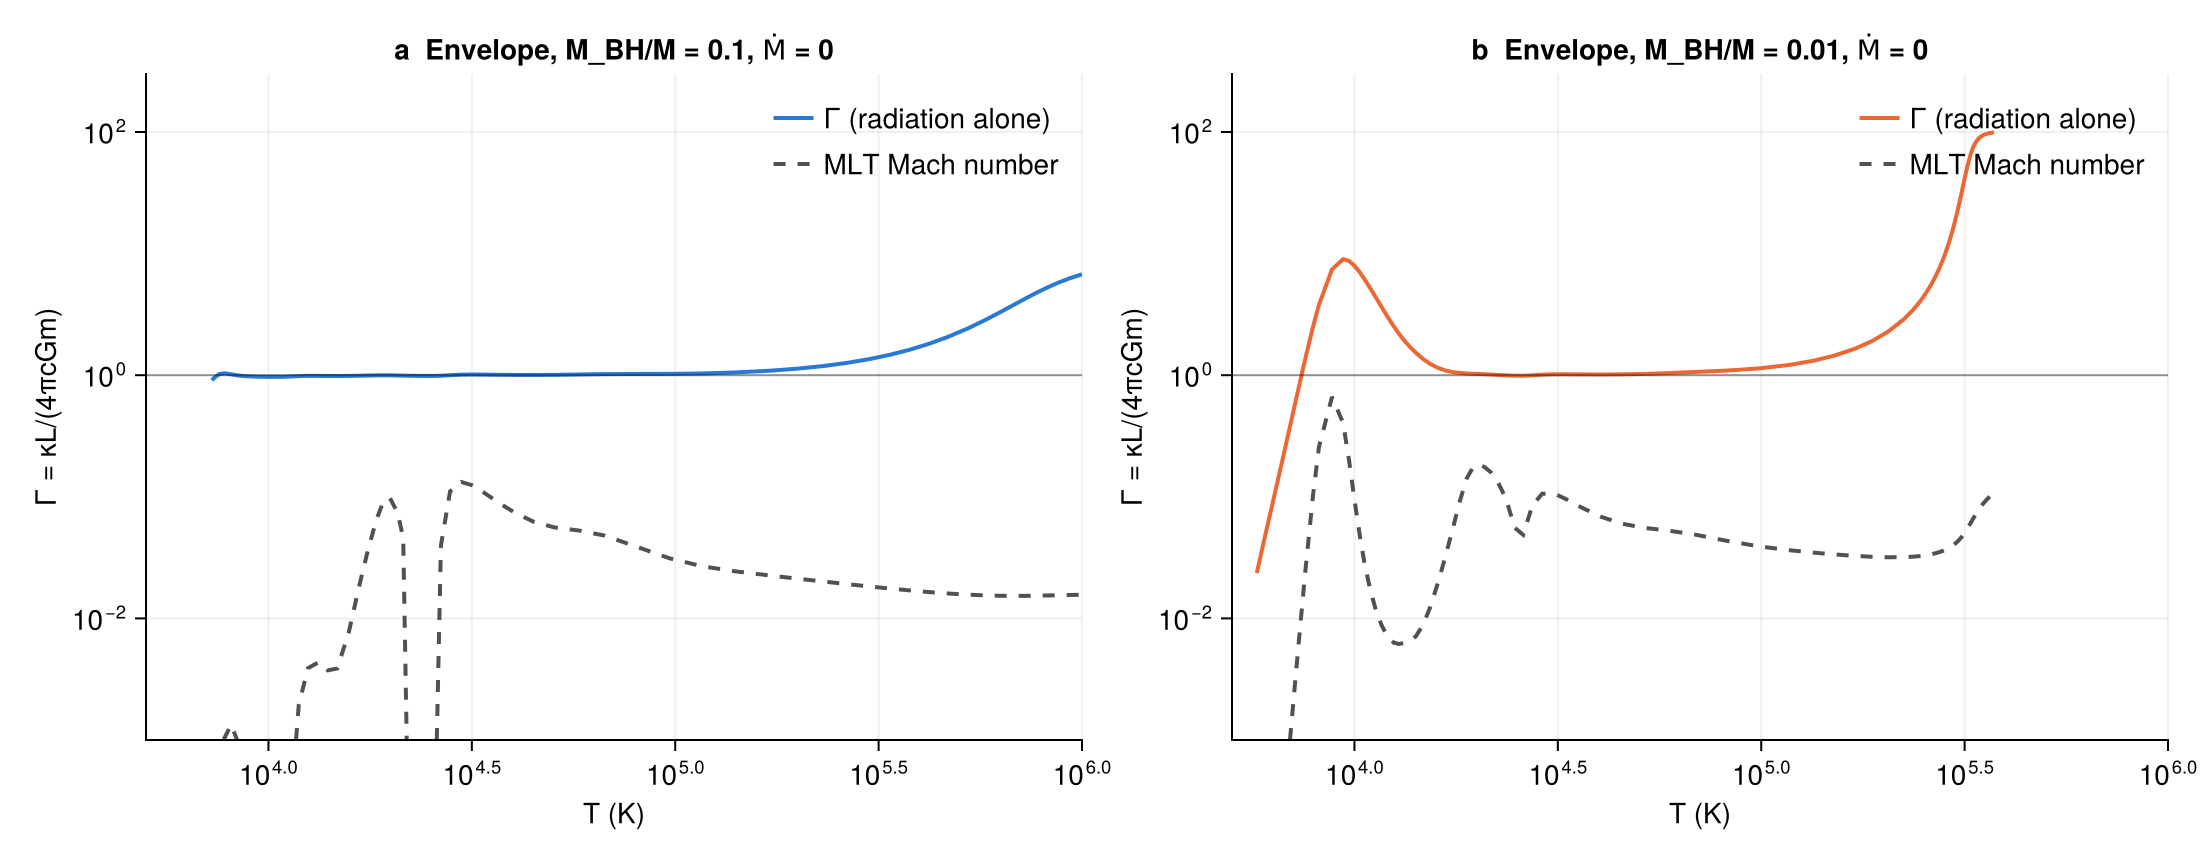
\includegraphics[width=\textwidth]{fig_envelope_profiles.png}
\caption{No-infall envelopes: local Eddington factor for radiation alone and MLT Mach number vs.\ temperature.}
\label{fig:prof}
\end{figure}

\subsection{With infall: two branches and a fold}\status{computed}
Scanning $\log R\in[14,16.6]$ in steps of 0.025 and bisecting every sign change gives the solutions in
Table~\ref{tab:br} and Fig.~\ref{fig:br}. (An earlier version of this analysis that kept only the first root
reported a spurious jump at $\Mdot\approx3$; it is superseded.)

\begin{table}[h]
\centering\small
\begin{tabular}{rrcccccc}
\toprule
$M_{\rm BH}/M$ & $\Mdot$ & branch & $R$ (cm) & $T_b$ (K) & $\tau_{\rm in}^{\rm LTE}$ & $r_{\rm ph}/R$ & $T_{\rm obs}$ (K)\\
\midrule
0.1 & 0   & --       & $8.47\times10^{15}$ & 7261  & 0    & 1    & 7261\\
0.1 & 0.3 & compact  & $3.03\times10^{14}$ & 52976 & 3.24 & 10.6 & 11958\\
    &     & extended & $8.44\times10^{15}$ & 7356  & 0.06 & 1    & 7276\\
0.1 & 1   & compact  & $8.27\times10^{14}$ & 35871 & 5.74 & 9.69 & 7592\\
    &     & extended & $8.42\times10^{15}$ & 7528  & 0.18 & 1    & 7294\\
0.1 & 3   & compact  & $2.33\times10^{15}$ & 22450 & 7.28 & 4.48 & 6656\\
    &     & extended & $8.37\times10^{15}$ & 8036  & 0.58 & 1    & 7342\\
0.1 & 5   & compact  & $3.63\times10^{15}$ & 18197 & 7.61 & 2.93 & 6602\\
    &     & extended & $8.30\times10^{15}$ & 8604  & 1.10 & 1.09 & 7082\\
0.1 & $\ge10$ & \multicolumn{6}{l}{no steady solution in $10^{14}$--$4\times10^{16}$\,cm}\\
\midrule
0.01 & 0   & --       & $1.35\times10^{16}$ & 5753  & 0     & 1    & 5753\\
0.01 & 0.3 & compact  & $2.48\times10^{14}$ & 59989 & 3.65  & 13.3 & 11829\\
     &     & extended & $1.35\times10^{16}$ & 5758  & 0.003 & 1    & 5754\\
0.01 & 1   & compact  & $6.52\times10^{14}$ & 41997 & 6.78  & 13.1 & 7382\\
     &     & extended & $1.35\times10^{16}$ & 5770  & 0.007 & 1    & 5763\\
0.01 & 3   & compact  & $1.86\times10^{15}$ & 26648 & 9.26  & 6.03 & 6465\\
     &     & extended & $1.34\times10^{16}$ & 5804  & 0.01  & 1    & 5790\\
0.01 & 10  & compact  & $5.28\times10^{15}$ & 15871 & 9.29  & 2.12 & 6489\\
     &     & extended & $1.30\times10^{16}$ & 5962  & 0.04  & 1    & 5918\\
0.01 & $\ge25$ & \multicolumn{6}{l}{no steady solution in $10^{14}$--$4\times10^{16}$\,cm}\\
\bottomrule
\end{tabular}
\caption{Steady solutions ($M=10^6\,\Msun$, $L=L_{\rm Edd}$). $\Mdot$ in $\Msun$\,yr$^{-1}$ (or $\Mdot/f$ for streams).
Fold refinement ($\Delta\log R=0.01$): for $M_{\rm BH}/M=0.1$ the two roots are at $\log R=15.825$ and 15.895 at
$\Mdot=9$ and absent at 10; for $0.01$ they are at 16.005 and 16.075 at $\Mdot=20$ and absent at 25.}
\label{tab:br}
\end{table}

\begin{figure}[t]
\centering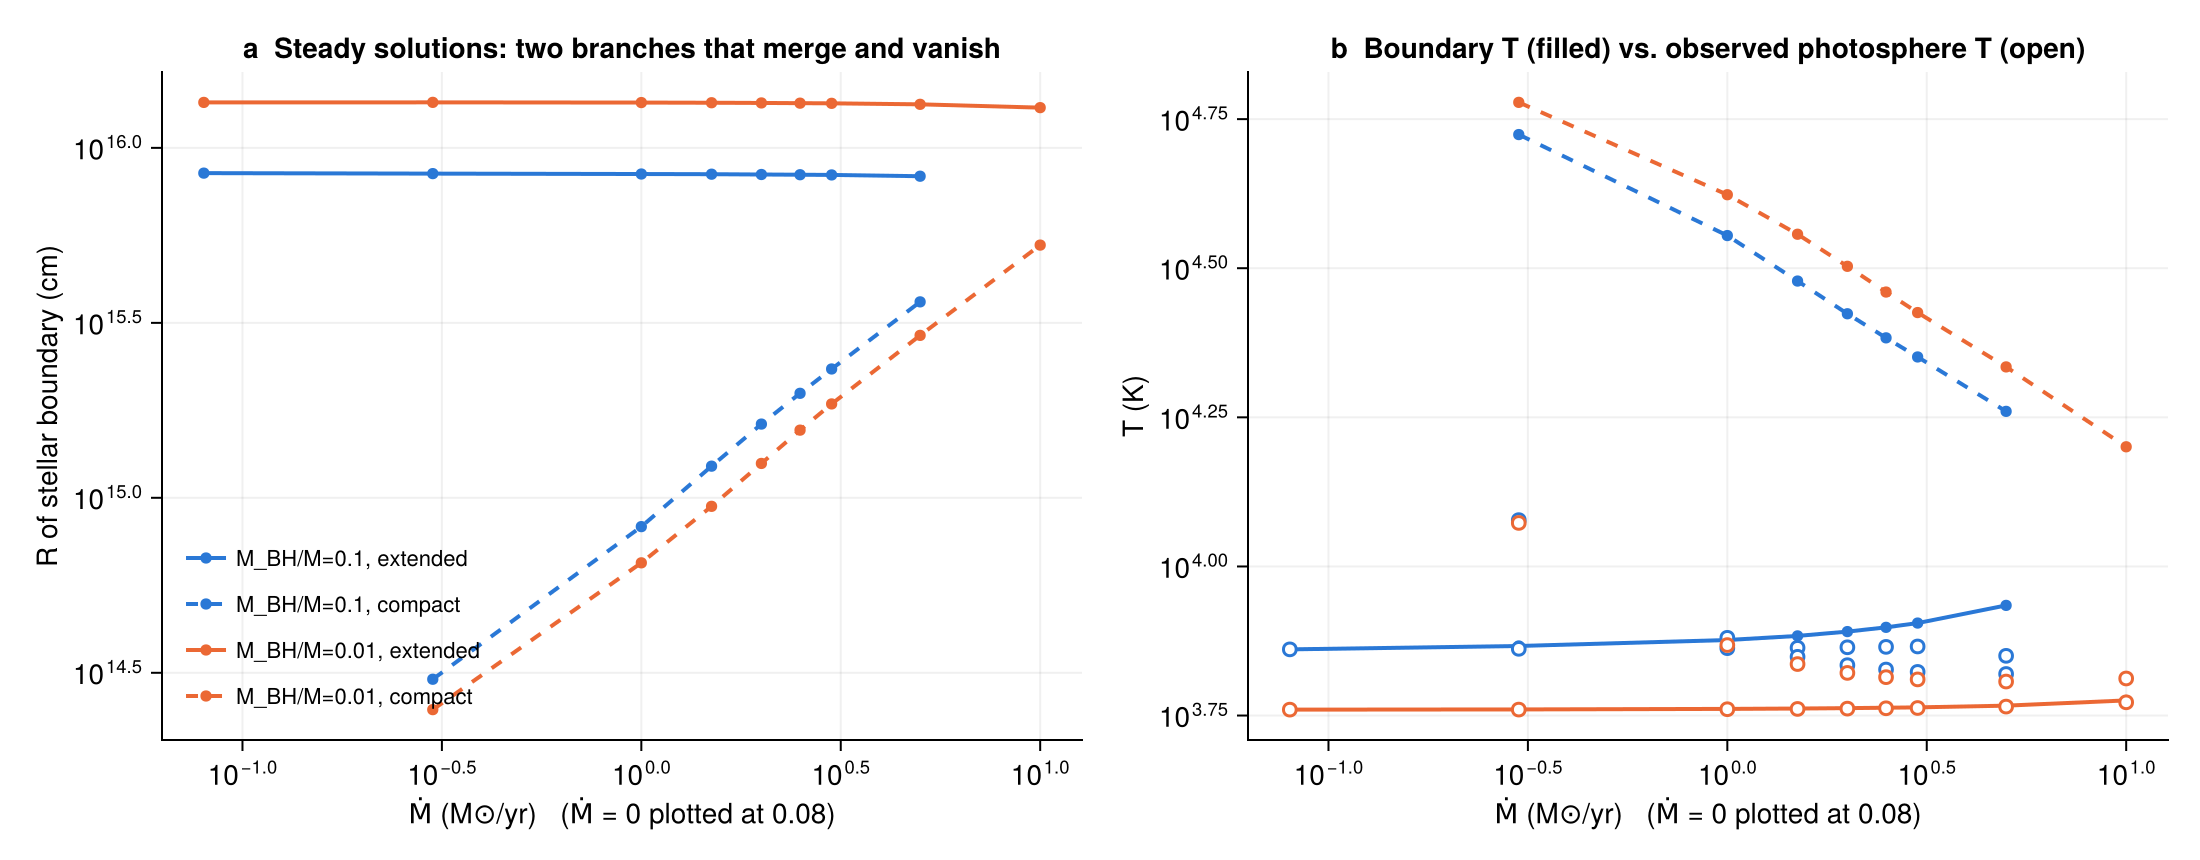
\includegraphics[width=\textwidth]{fig_branches.png}
\caption{(a) Stellar boundary radius of all steady solutions vs.\ $\Mdot$. (b) Boundary temperature (filled) and
observed-photosphere temperature (open; equal to $T_b$ when $\tau_{\rm in}<2/3$).}
\label{fig:br}
\end{figure}

\paragraph{Why infall cannot make a bigger star.} \status{interpretation, supported by the $\beta$ values above}
With $\beta\approx0.007$ nearly constant, the envelope is close to an Eddington standard model, whose mass fixes
$\beta$ and hence the adiabat (specific entropy). At fixed $M$ the adiabat is therefore pinned. The outer boundary
only selects where the adiabat is truncated. Ram pressure raises $P_b$, so the truncation moves deeper, to a higher
$(P,T)$, and the surface becomes smaller and hotter. Accretion-bloated protostars (Hosokawa et al.\ 2012, 2013) swell
for a different reason: entropy deposition in a gas-pressure-dominated star. That route is not available here.

\paragraph{What an observer sees.} On the compact branch the photosphere lies in the infall at $r_{\rm ph}\approx2$--13\,$R$,
i.e.\ $r_{\rm ph}\approx3\times10^{15}$--$1.1\times10^{16}$\,cm, approaching the extended-star radius for $\Mdot\ge1$. There $T_{\rm obs}\approx6400$--7600\,K, rising to
$\approx1.2\times10^4$\,K at $\Mdot=0.3$. \status{interpretation} The likely reason is that LTE hydrogen recombination
makes the opacity collapse near 6--7\,kK wherever the gas sits, so both branches show a 6000--7500\,K surface for $\Mdot\gtrsim1$. On the
compact branch, however, it is an infalling (several hundred km\,s$^{-1}$), X-ray-irradiated layer, not a hydrostatic
photosphere. Lines should be redshifted, and LTE is least justified there.

\paragraph{Confined super-Eddington layers.} At the boundary, $\Gamma_\kappa=\kappa_bF/(cg)$ exceeds unity on the compact
branch (1.4--3.9) and on the $M_{\rm BH}/M=0.1$ extended branch for $\Mdot\ge1$ (1.15--5.8). These layers are hydrostatic
only because the infall's ram pressure holds them down, a configuration expected to be Rayleigh--Taylor unstable
\status{interpretation}.

\begin{figure}[t]
\centering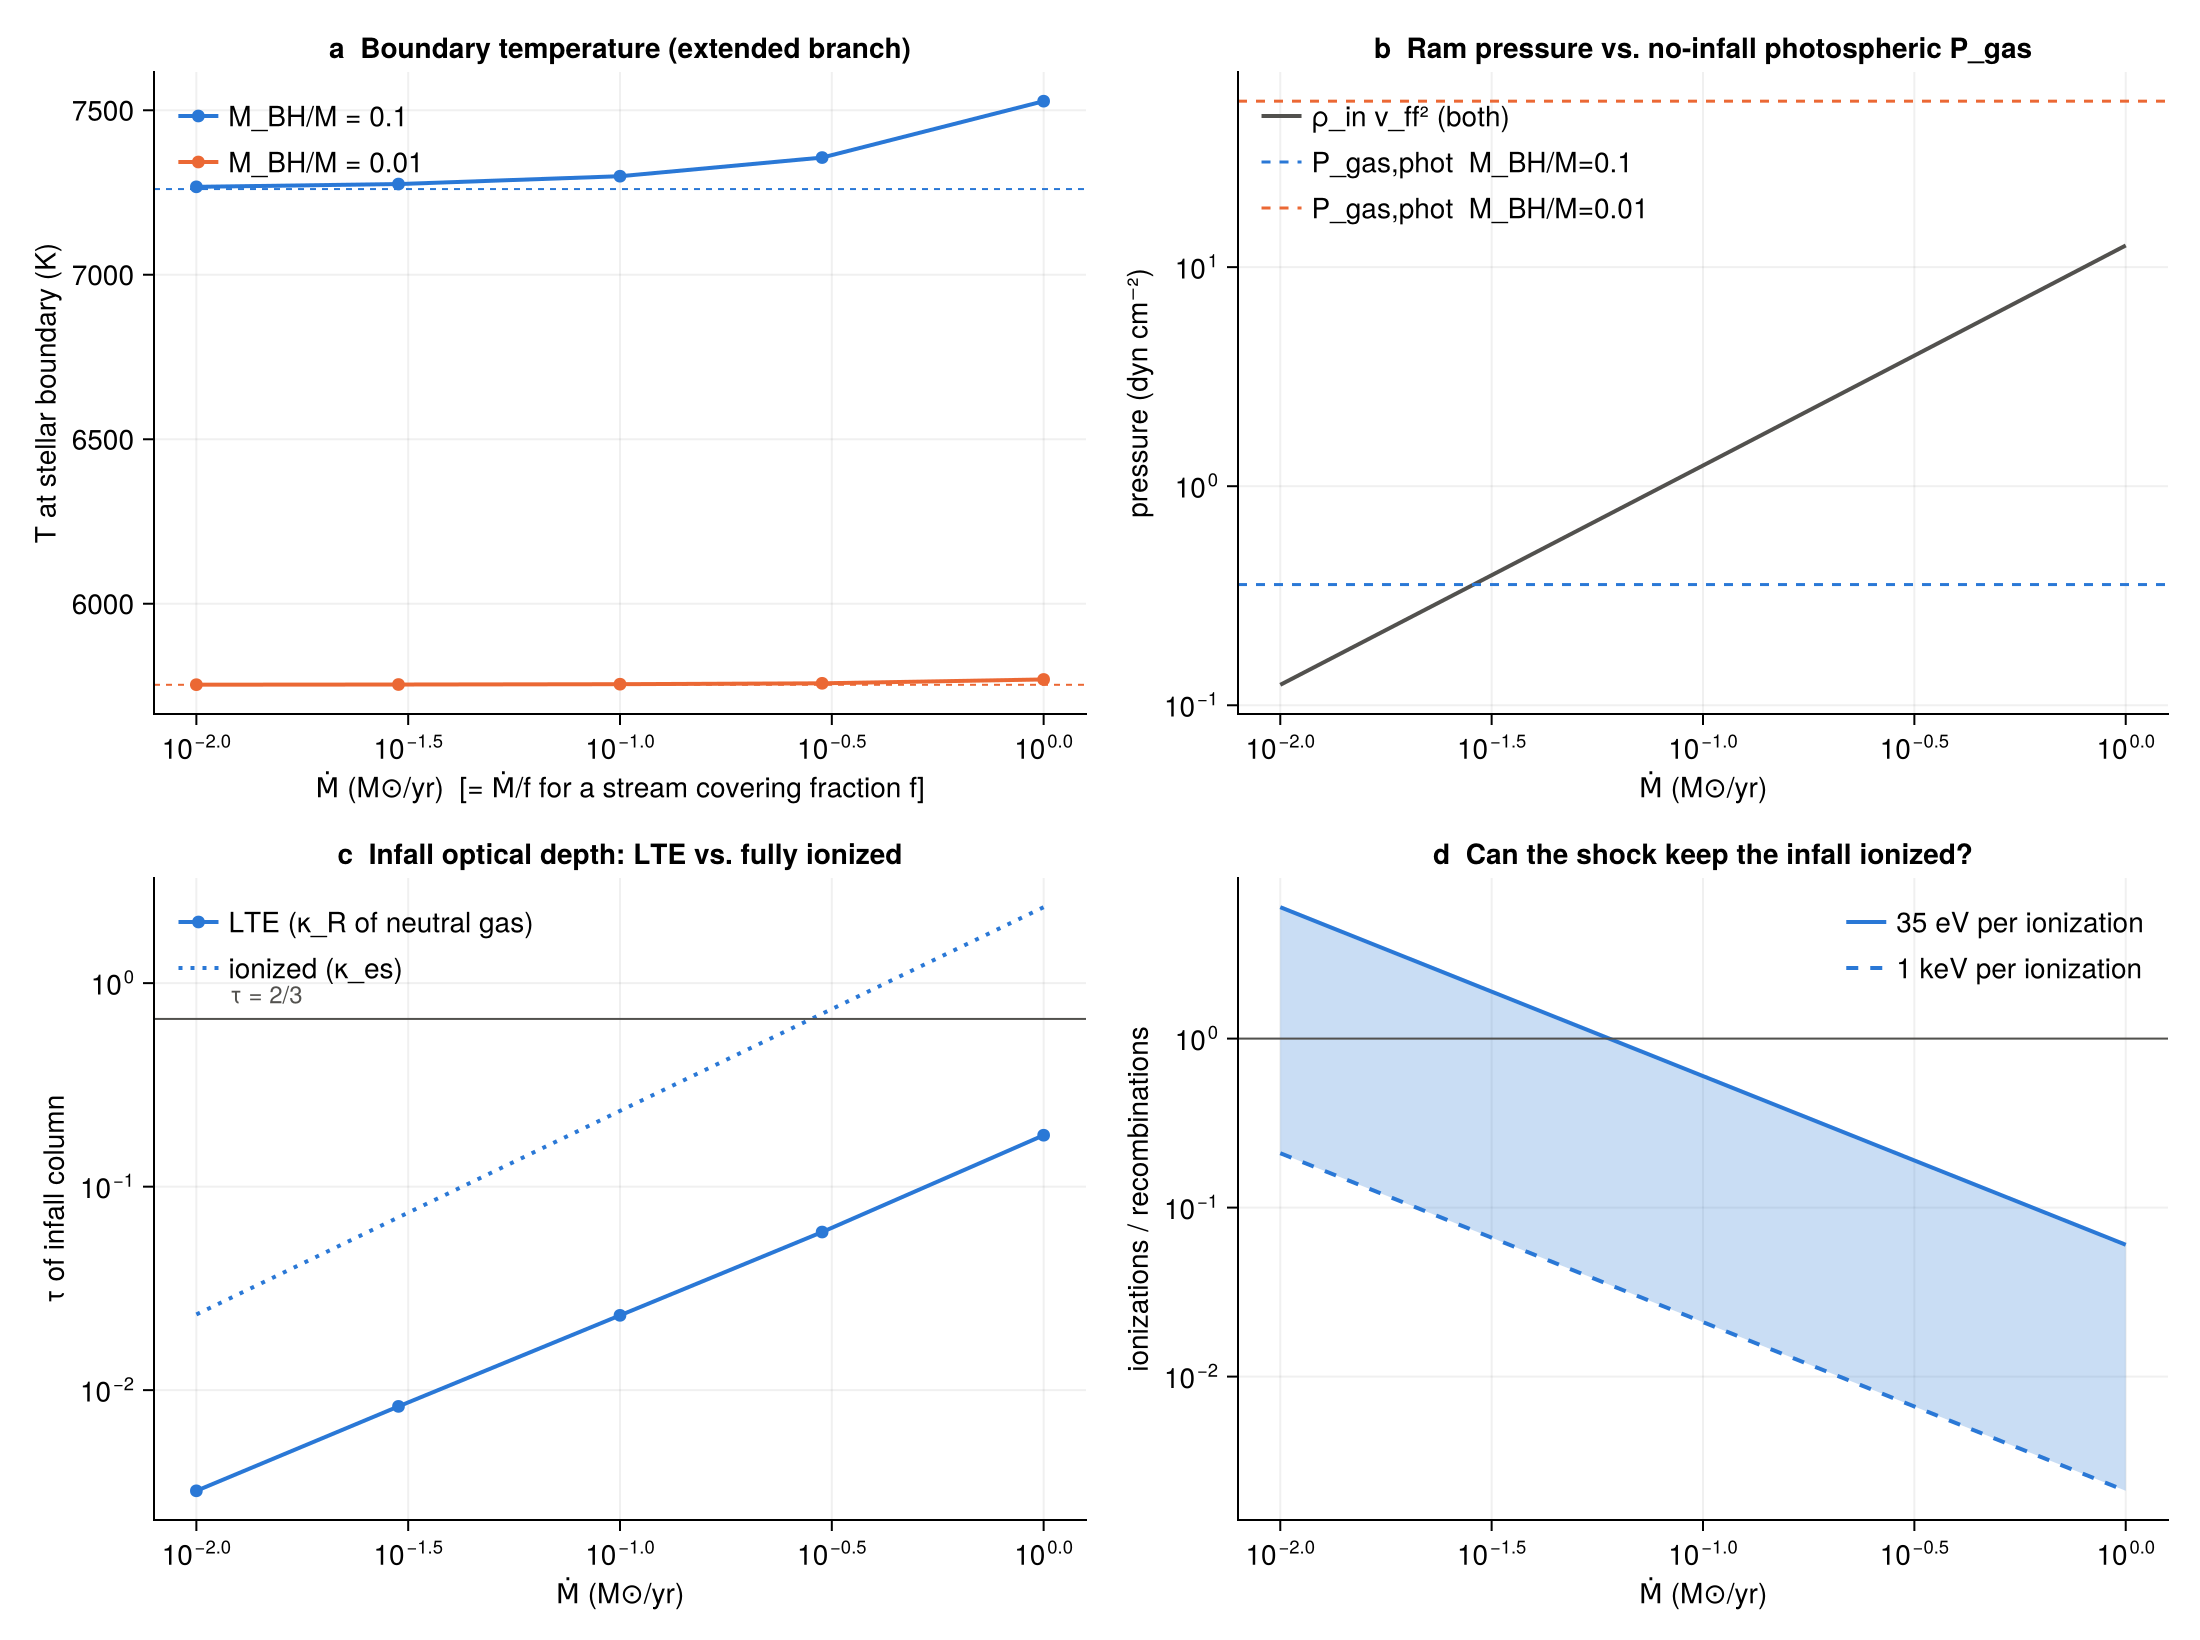
\includegraphics[width=\textwidth]{fig_infall_boundary.png}
\caption{Extended-branch diagnostics vs.\ $\Mdot$. (a) Boundary temperature. (b) Ram pressure vs.\ photospheric gas pressure
without infall. (c) Infall optical depth, LTE vs.\ fully ionized. (d) Ratio of ionizations driven by the shock to recombinations in the infall
($\le10R$), bracketed by 35\,eV and 1\,keV per ionization.}
\label{fig:diag}
\end{figure}

\subsection{Infall diagnostics on the extended branch}\status{estimate}
For $M_{\rm BH}/M=0.1$:
\begin{center}
\begin{tabular}{rcccccc}
\toprule
$\Mdot$ & $\rho_{\rm in}v_{\rm ff}^2$ (dyn\,cm$^{-2}$) & $\tau_{\rm in}^{\rm LTE}$ & $\tau_{\rm in}^{\rm es}$ & $\ell_{\rm cool}/R$ & ion/rec (35\,eV--1\,keV) & $\Gamma_{\rm es}$\\
\midrule
0.01 & 0.12 & 0.003 & 0.024 & 0.37  & 6.0--0.21   & 1.0001\\
0.03 & 0.37 & 0.008 & 0.071 & 0.12  & 2.0--0.07   & 1.0002\\
0.1  & 1.24 & 0.023 & 0.24  & 0.037 & 0.60--0.021 & 1.0007\\
0.3  & 3.74 & 0.060 & 0.71  & 0.012 & 0.20--0.007 & 1.0021\\
1    & 12.6 & 0.18  & 2.4   & 0.004 & 0.06--0.002 & 1.0070\\
\bottomrule
\end{tabular}
\end{center}
These numbers raise two consistency issues that the steady model cannot resolve.
\begin{enumerate}
\item Because $L\ge L_{\rm Edd}(\kes)$, \emph{ionized} infall is weightless or pushed outward, so it cannot be in free fall. Free-fall
infall must be largely neutral.
\item Whether the shock keeps the infall ionized depends on the energy per ionization. At low $\Mdot$ it likely does; at high
$\Mdot$ recombinations ($\propto\Mdot^2$) outrun ionizations ($\propto\Mdot$). On the compact branch the gas near the shock
is at 16--60\,kK and ionized, so the free-fall boundary is internally inconsistent there. The thin-shock assumption fails
for $\Mdot\lesssim0.03$ ($\ell_{\rm cool}/R\gtrsim0.1$).
\end{enumerate}

\section{Limitations}
\begin{itemize}
\item 1D, spherical, steady; local MLT (not TDC); no turbulent pressure; no rotation.
\item LTE throughout, including the infall. Photoionization by the $\sim3\times10^7$\,K shock is ignored except in the budget
estimate. The radiation force on the infall is ignored in the boundary condition.
\item Continuum-only Rosseland opacity (no H/He lines, no molecules).
\item Inner boundary is a point mass with $m(\varepsilon_{\rm in}R)=M_{\rm BH}$, not the MESA-QUEST saturated-convection radius.
\item Stability of the two branches has not been analysed. Which one nature selects, and what happens past the fold, requires
dynamics.
\item The §\ref{sec:nlte} rate comparisons use textbook approximations and are good to a factor of a few.
\end{itemize}

\section{Next steps}
\begin{enumerate}
\item Linear stability of both branches. This is cheap and tells the dynamical runs what to look for.
\item Dynamical radiation hydrodynamics: TITAN (Gehmeyr \& Mihalas 1994). The 1995 Fortran release now builds with gfortran; all
benchmarks run, and the six with a fixed end time reproduce the 1995 step counts exactly. It runs as a shared library driven from Julia, bitwise identical to the
standalone code. A Julia port (tolerance-verified, not bitwise) is under way. TITAN has no convection; a time-dependent
convection model must be added.
\item Time-independent NLTE post-processing (H with 10--15 levels plus continuum, then He) on steady and dynamical snapshots. This is justified because
recombination times ($\sim10$\,s at the photosphere, $\lesssim1$\,d in the infall) are $\ll R/v_{\rm ff}\sim2$\,yr. The first target is
the Balmer break on both branches.
\end{enumerate}

\section*{Code and data}\sloppy
\texttt{QuasiStarInfall.jl} (Julia 1.11): \texttt{src/} (EOS, opacity, envelope, boundary) and \texttt{scripts/}
(\texttt{build\_kap.jl}, \texttt{validate2.jl}, \texttt{run\_grid.jl}, \texttt{branches.jl}, \texttt{fold.jl}, \texttt{plot\_grid.jl}).
Results are in \texttt{output/*.csv}.

\section*{References}
{\small
\begin{itemize}[leftmargin=*,label={}]
\item Ball W.\,H., Tout C.\,A., \.Zytkow A.\,N., Eldridge J.\,J.\ 2011, MNRAS 414, 2751
\item Begelman M.\,C., Rossi E.\,M., Armitage P.\,J.\ 2008, MNRAS 387, 1649
\item Begelman M.\,C., Dexter J.\ 2025, arXiv:2507.09085
\item Campbell C.\,B., Santarelli A.\,D., Caplan M.\,E.\ 2025, RNAAS 9, 185
\item Castelli F., Kurucz R.\,L.\ 2003, IAU Symp.\ 210, A20
\item Coughlin E.\,R., Begelman M.\,C.\ 2024, arXiv:2405.00084
\item Gehmeyr M., Mihalas D.\ 1994, Physica D 77, 320
\item Hosokawa T., Omukai K., Yorke H.\,W.\ 2012, ApJ 756, 93
\item Hosokawa T.\ et al.\ 2013, ApJ 778, 178
\item Inayoshi K., Hosokawa T., Omukai K.\ 2013, MNRAS 431, 3036
\item Jiang Y.-F.\ et al.\ 2015, ApJ 813, 74
\item John T.\,L.\ 1988, A\&A 193, 189
\item Kippenhahn R., Weigert A., Weiss A., \emph{Stellar Structure and Evolution}, 2nd ed.
\item Lucy L.\,B.\ 1971, ApJ 163, 95
\item Naidu R.\,P.\ et al.\ 2025, arXiv:2503.16596
\item Santarelli A.\,D.\ et al.\ 2026a, ApJ 998, 150 (MESA-QUEST)
\item Santarelli A.\,D.\ et al.\ 2026b, ApJL 998, L4
\item Sincell M.\,W., Gehmeyr M., Mihalas D.\ 1999, Shock Waves 9, 391; 403
\end{itemize}}
\end{document}
